\documentclass[letterpaper,twocolumn,10pt]{article}
\usepackage{usenix2019_v3}

% figures and tables
\usepackage{graphicx}
\usepackage{subcaption}
\usepackage{booktabs}
\usepackage{multirow}
\usepackage{array}
\usepackage{siunitx}
\sisetup{group-separator={,}, group-minimum-digits=4}
\usepackage{tikz}
\usetikzlibrary{positioning,arrows.meta,fit,calc,shapes.geometric,shapes.misc,patterns,decorations.pathreplacing,backgrounds}
\usepackage[most]{tcolorbox}

% math
\usepackage{amsmath,amssymb}
\usepackage{amsthm}

% text
\usepackage{listings}
\lstset{basicstyle=\ttfamily\scriptsize,breaklines=true,columns=fullflexible}
\usepackage{enumitem}
\setlist{nosep,leftmargin=*}
\usepackage{xspace}
\usepackage[capitalise,noabbrev]{cleveref}

\hypersetup{pdfauthor={},pdftitle={Pin, Replay, or Refuse},colorlinks=true,linkcolor=blue!50!black,citecolor=blue!50!black,urlcolor=blue!50!black}

\theoremstyle{definition}
\newtheorem{definition}{Definition}
\newtheorem{assumption}{Assumption}

% palette shared with figures/make_figures.py
\definecolor{cStable}{HTML}{9ECAE1}
\definecolor{cEdited}{HTML}{FD8D3C}
\definecolor{cNew}{HTML}{E6550D}
\definecolor{cTare}{HTML}{2171B5}
\definecolor{cReplay}{HTML}{6BAED6}
\definecolor{cOk}{HTML}{31A354}
\definecolor{cBad}{HTML}{CB181D}
\definecolor{cGrey}{HTML}{636363}

% plain-language callout box
\newtcolorbox{plainbox}[1]{enhanced,breakable,colback=cTare!4,colframe=cTare!70!black,boxrule=0.5pt,arc=1.5pt,
  left=4pt,right=4pt,top=3pt,bottom=3pt,fonttitle=\bfseries\small,title={#1},fontupper=\small}

\newcommand{\sys}{TARE\xspace}
\newcommand{\pending}[1]{\textcolor{red}{[PENDING: #1]}}
\newcommand{\tbd}{\textcolor{red}{TBD}}
\newcommand{\dec}[1]{\textsc{#1}}
\newcommand{\cutga}{\texttt{-{}-cut\_ga}\xspace}

\title{Pin, Replay, or Refuse: Exact Incremental Re-annotation\\
Across Reference Database Releases}
\author{Anonymous Submission}
\date{}

\begin{document}
\maketitle

% =====================================================================
\begin{abstract}
Biologists label the genes in a new genome by comparing them against large public reference databases such
as Pfam, UniProt, and InterPro. Those databases publish new versions every few weeks to months, and each new
version forces laboratories to redo the comparison from scratch, even though most of the database has not
changed: 86.6\% of Pfam's entries were identical between versions 38.1 and 38.2.
% source: MEASURED pipeline/results/reference_kill_r1.json unchanged_strict=26082 z_new=30134; HAS 38.1; HAS 38.2; DERIVED identical_pct=100*unchanged_strict/z_new
Reusing the old results
is harder than skipping the unchanged entries, because the search programs are fixed binaries and the
statistics they print depend on the size of the whole database. Rerunning the standard tool, HMMER, on
exactly the right entries without accounting for this changes 99.9\% of its output lines.
% source: MEASURED pipeline/results/exact_replay/e1scale.json proteomes.0.Rn.vs_stock.tbl.differing_positions=9083 proteomes.0.Rn.vs_stock.tbl.lines_stock=9094; DERIVED one_pct=100*differing_positions/lines_stock

We present \sys (Tool Annotation Reuse, Exact). \sys rests on one observation: in these programs, the way
one database entry affects another is concentrated in a few numbers, such as the database size, that the
program already lets a user set. \sys finds those numbers by experimenting on the program from the outside,
fixes (``pins'') them to the new version's values, and reruns the unmodified program only on what can
change, so the program itself prints output that is byte-for-byte identical to a full rerun. When a cheap
check cannot rule out a hidden dependency, \sys refuses and runs the program in full instead. Across
92{,}595 output lines from two programs, every result \sys produced was identical to a full rerun. On a Pfam update, \sys is \pending{X$\times$ (server, median of ten genomes)} faster than a full rerun (3.4$\times$ on a
workstation, geometric mean of two genomes),
general-purpose caches reuse nothing, and an existing incremental search tool matched a full run on only
1.3\% of its rows.
% source: MEASURED pipeline/results/exact_replay/e1_e2.json E1.check1_R_vs_S.tbl.lines_a=534 E1.check1_R_vs_S.dom.lines_a=545; MEASURED pipeline/results/exact_replay/e1scale.json tblout_body_lines_total=26127 proteomes.0.domtblout_body_lines=8812 proteomes.1.domtblout_body_lines=8202 proteomes.2.domtblout_body_lines=8265; MEASURED pipeline/results/exact_replay/costpass_measured.json proteomes.0.e2.tbl.lines_stock=8714 proteomes.1.e2.tbl.lines_stock=9291 proteomes.0.e2.dom.lines_stock=8405 proteomes.1.e2.dom.lines_stock=9024 proteomes.0.stock.wall_s=648.9416185829905 proteomes.0.e2.wall_s=190.69520458299667 proteomes.1.stock.wall_s=693.2145589159918 proteomes.1.e2.wall_s=205.20091079198755; MEASURED pipeline/results/infernal/test_i.json rows.noclan=4217; MEASURED pipeline/docs/INFERNAL_PROTOCOL.md; TEXT shipped_rows=459; MEASURED pipeline/results/reference_diamond/dx.json dx_i.idiamond.shared_byte_identical=407 dx_i.idiamond.shared_rows=31377; DERIVED n_lines=E1_check1_R_vs_S_tbl_lines_a+E1_check1_R_vs_S_dom_lines_a+tblout_body_lines_total+proteomes_0_domtblout_body_lines+proteomes_1_domtblout_body_lines+proteomes_2_domtblout_body_lines+proteomes_0_e2_tbl_lines_stock+proteomes_1_e2_tbl_lines_stock+proteomes_0_e2_dom_lines_stock+proteomes_1_e2_dom_lines_stock+noclan+shipped_rows; DERIVED s0=proteomes_0_stock_wall_s/proteomes_0_e2_wall_s; DERIVED s1=proteomes_1_stock_wall_s/proteomes_1_e2_wall_s; DERIVED gmean=geomean(s0,s1); DERIVED ident_pct=100*shared_byte_identical/shared_rows
\end{abstract}

% =====================================================================
\section{Introduction}
\label{sec:intro}

When a laboratory sequences a genome, it obtains thousands of protein sequences with no labels. To learn what
each protein does, researchers compare it against \textit{reference databases}: curated collections of known
protein families, such as Pfam~\cite{pfam2025}, UniProt~\cite{uniprot2025}, and InterPro~\cite{paysanlafosse2023interpro}.
A program such as HMMER~\cite{eddy2011hmmer} scores every protein against every family and reports the good
matches, called \textit{hits}. This step, called \textit{annotation}, underlies much of modern biology, from
comparative genomics to the sequence alignments used by structure predictors such as AlphaFold~\cite{jumper2021alphafold}.

Reference databases keep improving. UniProt and InterPro publish a new version, called a \textit{release},
roughly every eight weeks~\cite{uniprot2025,paysanlafosse2023interpro}, and Pfam published eight releases
between May 2024 and June 2026~\cite{pfam382relnotes}. Each release adds and revises families, so annotations
computed against an old release go out of date. The annotation programs keep no memory of earlier runs,
so the only way to update is to compare every protein against the entire new database again. Most of that
work recomputes answers that did not change: between Pfam 38.1 and 38.2, 86.6\% of the 30{,}134 families were
byte-for-byte identical (\cref{fig:churn}). At scale this repeated cost shapes practice. NCBI re-annotates its
RefSeq collection on a rolling schedule because redoing all of it at once ``requires securing at once a
significant amount of computing resources''~\cite{li2021refseq}, and JGI states that at over 65 billion genes
``it is impossible to upgrade all genome and metagenome annotations to the latest version''~\cite{chen2021img}.
% source: CITED pipeline/docs/MOTIVATION_EVIDENCE.md; yy:05/24=2024; yy:06/26=2026; TEXT genes_b=65; HAS 38.1; HAS 38.2; MEASURED pipeline/results/reference_kill_r1.json z_new=30134 unchanged_strict=26082; DERIVED identical_pct=100*unchanged_strict/z_new

\begin{figure*}[t]
\centering
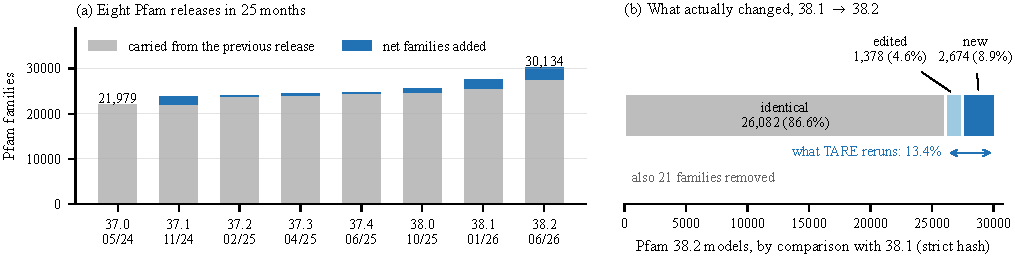
\includegraphics[width=\textwidth]{figures/churn.pdf}
\caption{\textbf{Reference databases change often, but mostly stay the same.} (a) Pfam grew from 21{,}979 to
30{,}134 families over eight releases; orange bars show how many families each release added. (b) Comparing
every model of Pfam 38.2 with 38.1 byte for byte: 86.6\% are identical. Only 13.4\% (new or edited) can produce
new results, yet a conventional update recomputes 100\%.}
% source: CITED pipeline/docs/MOTIVATION_EVIDENCE.md; TEXT fam_37_0=21979; TEXT fam_38_2=30134; HAS 38.1; HAS 38.2; MEASURED pipeline/results/reference_kill_r1.json z_new=30134 unchanged_strict=26082; DERIVED identical_pct=100*unchanged_strict/z_new; DERIVED changed=z_new-unchanged_strict; DERIVED changed_pct=100*changed/z_new; DERIVED full_pct=100*z_new/z_new
\label{fig:churn}
\end{figure*}

\textbf{Why reuse is hard.} It might seem easy to search only the new and edited families and keep the old results
for the rest. It is not, for three reasons. First, the results are \textit{coupled}: the statistic HMMER prints for
each hit, its E-value, is scaled by the total number of families in the database, much as a grade curved to class
size changes for every student when new students enroll. Adding families therefore changes the printed numbers of
hits on families that did not change. Rerunning HMMER on exactly the right families, without accounting for this,
changes 9{,}083 of 9{,}094 output lines for one bacterial genome.
% source: MEASURED pipeline/results/exact_replay/e1scale.json proteomes.0.Rn.vs_stock.tbl.differing_positions=9083 proteomes.0.Rn.vs_stock.tbl.lines_stock=9094
Second, the programs are unmodified binaries
maintained by others; we cannot change their code. Third, an approximately correct answer is not good enough:
pipelines that track provenance must reproduce a full run exactly, because ``pipeline differences can lead to
annotation discrepancies''~\cite{chen2021img}.

Existing tools fall short in two ways. General-purpose caches, such as build systems and workflow
managers~\cite{curtsinger2022riker,xie2026incr,shiptoski2023processcache,ditommaso2017nextflow,molder2021snakemake},
remember whole commands keyed by the bytes they read. A new release changes the database file, so they rerun the
search in full. Specialized incremental search tools such as iBLAST and iSeqSearch~\cite{dash2021iblast,yoo2025iseqsearch}
are written by hand for one program and adjust the printed numbers after the fact. Their output is approximate, and
they cannot tell when their adjustment is wrong: in our experiment, only 1.3\% of the rows that iSeqSearch shared
with a full run were byte-identical, and it reported 133 hits to sequences that the new release had deleted.
% source: MEASURED pipeline/results/reference_diamond/dx.json dx_i.idiamond.shared_byte_identical=407 dx_i.idiamond.shared_rows=31377 dx_i.idiamond.row_extra=133; DERIVED ident_pct=100*shared_byte_identical/shared_rows
\textit{How can we reuse earlier annotations across a database release, without modifying the programs, while
guaranteeing exactly the output of a full rerun?}

\begin{plainbox}{The key idea in plain terms}
In the programs we studied, entries in the database influence each other's printed results through only a few
global numbers, chiefly the database size, and the programs already accept those numbers as settings. If we tell
the program the new release's size up front (\textit{pin} it), it scores each family on its own merits. Then we can
rerun it on a small subset of the database and it prints exactly what a full run would print, digit for digit,
because the program, not our wrapper, computes every number. When a program breaks this pattern, we can detect it
and fall back to a full run.
\end{plainbox}

Building on this idea, we present \sys, a wrapper that sits in front of an unmodified annotation program. \sys
first learns, by running the program on carefully chosen pieces of the database, how its output splits across
database entries and which global numbers tie them together (\cref{sec:contract}). It then pins those numbers to the
new release, finds new hits on the changed families, and reruns the program on each protein's few candidate families
(\cref{sec:replay}). Before returning anything, \sys runs a check that adds back families the rerun left out and
refuses if any line changes (\cref{sec:check}). Every refusal falls back to an ordinary full run, so users always
receive the program's own output.

We evaluate \sys on four programs: two where it reproduces full runs exactly (HMMER and Infernal) and two where it
correctly refuses (DIAMOND and BLAST+). Our contributions are:
\begin{enumerate}
  \item \textbf{Black-box coupling inference.} A method that discovers, with no program-specific code, how a program's
  output decomposes over database entries and which quantities couple them (\cref{sec:contract,sec:gate}).
  \item \textbf{Exact replay with check-or-refuse.} Pinned, batched replay that makes an unmodified program print
  byte-identical output, and a check that refuses when replay is unsafe. Investigating a failure of our first check
  revealed why DIAMOND cannot be replayed exactly: its first filter reads bytes belonging to the neighboring
  database entry (\cref{sec:eval-safety}).
  \item \textbf{A predictive cost model and a pre-registered evaluation.} A simple formula for how much faster an update
  can be, which predicts the dominant cost within 7.1\% (\cref{sec:cost}), and experiments whose design and pass/fail
% source: MEASURED pipeline/results/exact_replay/costpass_measured.json proteomes.0.stock.wall_s=648.9416185829905 proteomes.0.e2.phases.discovery_s=91.15112141700229 proteomes.1.stock.wall_s=693.2145589159918 proteomes.1.e2.phases.discovery_s=100.30562595801894; MEASURED pipeline/results/reference_kill_r1.json z_new=30134 unchanged_strict=26082; DERIVED f_delta=(z_new-unchanged_strict)/z_new; DERIVED pred0=f_delta*proteomes_0_stock_wall_s; DERIVED pred1=f_delta*proteomes_1_stock_wall_s; DERIVED err0=abs(pred0-proteomes_0_e2_phases_discovery_s)/proteomes_0_e2_phases_discovery_s; DERIVED err1=abs(pred1-proteomes_1_e2_phases_discovery_s)/proteomes_1_e2_phases_discovery_s; DERIVED err_pct=100*err1
  rules were committed before they ran (\cref{sec:eval}).
\end{enumerate}

% =====================================================================
\section{Background}
\label{sec:background}

\begin{table}[t]
\caption{Terms used in this paper.}
\label{tab:glossary}
\centering\footnotesize
\setlength{\tabcolsep}{3pt}
\begin{tabular}{@{}>{\raggedright\arraybackslash}p{1.6cm}>{\raggedright\arraybackslash}p{6.2cm}@{}}
\toprule
Term & Meaning \\
\midrule
Record & One query item, here one protein (or one DNA sequence for Infernal). \\
Reference & The database searched against, here Pfam or Rfam; a file of \textit{entries}. \\
Entry & One family model in the reference (a profile HMM in Pfam). \\
Release & A new version of the reference. \\
Hit / row & A reported record--entry match; one line of the output table. \\
E-value & How many matches this good would be expected by chance in the whole database; scaled by the database size $Z$. \\
Stock run & Running the unmodified program on everything, the result we must reproduce. \\
Pin & Fixing a global setting (e.g., $Z$) to the new release's value. \\
Replay & Rerunning the unmodified program on a subset of the reference. \\
\bottomrule
\end{tabular}
\end{table}

\subsection{How Annotation Works}

An annotation program takes two inputs: a set of \textit{records}, such as the thousands of proteins of a bacterial
genome, and a \textit{reference} of \textit{entries}, such as Pfam's 30{,}134 protein families (\cref{tab:glossary}).
% source: MEASURED pipeline/results/reference_kill_r1.json z_new=30134
Each Pfam family is stored as a statistical profile, a profile hidden Markov model, that summarizes what members
of that family look like. HMMER's \texttt{hmmscan} compares every protein with every family, computes a score, and
writes one line per reported hit, containing the names of the protein and family, the score, and an E-value. The
E-value estimates how many equally good matches would occur by chance in a database of this size, and HMMER computes
it as a probability multiplied by $Z$, the number of families in the database~\cite{eddy2011hmmer}. With Pfam's curated
per-family score thresholds (the \cutga option), whether a hit is reported depends only on its score against that
family's threshold~\cite{pfam2025}.

\subsection{Why Naive Reuse Fails}

\begin{figure}[t]
\centering
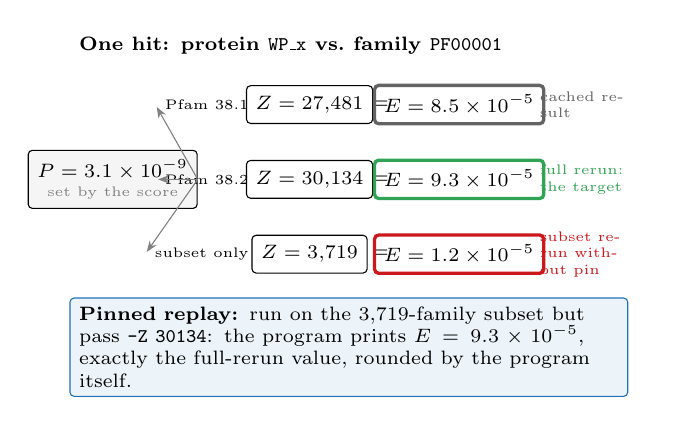
\begin{tikzpicture}[font=\scriptsize, x=1cm, y=1cm]
  \node[anchor=west, font=\scriptsize\bfseries] at (-0.1,3.0) {One hit: protein \texttt{WP\_x} vs.\ family \texttt{PF00001}};
  \node[draw, rounded corners=1.5pt, fill=gray!8, minimum width=1.35cm, minimum height=0.6cm, align=center] (P) at (0.45,1.3)
     {$P = 3.1\times10^{-9}$\\[-1pt]{\tiny\color{gray} set by the score}};
  \foreach \y/\nm/\lab/\z/\e/\col/\note in {
     2.25/ZA/Pfam 38.1/27{,}481/8.5\times10^{-5}/cGrey/cached result,
     1.30/ZB/Pfam 38.2/30{,}134/9.3\times10^{-5}/cOk/full rerun: the target,
     0.35/ZC/subset only/3{,}719/1.2\times10^{-5}/cBad/subset rerun without pin}{
% source: DATAONLY ILLUSTRATIVE GIVEN p=3.1e-9; MEASURED pipeline/results/reference_kill_r1.json z_old=27481 z_new=30134; HAS 38.1; HAS 38.2; MEASURED pipeline/results/exact_replay/e1scale.json proteomes.0.candidate_models_E1=3719; DERIVED e_old=p*z_old; DERIVED e_new=p*z_new; DERIVED e_sub=p*candidate_models_E1
     \node[anchor=east, font=\tiny] (L\nm) at (2.3,\y) {\lab};
     \node[draw, rounded corners=1.5pt, minimum width=1.25cm, minimum height=0.48cm] (\nm) at (2.95,\y) {$Z = \z$};
     \node at (3.85,\y) {$=$};
     \node[draw=\col, very thick, rounded corners=1.5pt, minimum width=1.7cm, minimum height=0.48cm] at (4.85,\y) {$E = \e$};
     \node[anchor=west, text=\col, font=\tiny, text width=1.25cm, align=left] at (5.75,\y) {\note};
     \draw[-{Stealth[length=1.4mm]}, gray, shorten >=1pt] (P.east) -- (L\nm.west);
  }
  \node[draw=cTare, fill=cTare!8, rounded corners=1.5pt, align=left, anchor=north west, text width=6.85cm] at (-0.1,-0.2)
  {\textbf{Pinned replay:} run on the 3{,}719-family subset but pass \texttt{-Z 30134}: the program prints
   $E = 9.3\times10^{-5}$, exactly the full-rerun value, rounded by the program itself.};
% source: DATAONLY ILLUSTRATIVE GIVEN p=3.1e-9; MEASURED pipeline/results/reference_kill_r1.json z_new=30134; MEASURED pipeline/results/exact_replay/e1scale.json proteomes.0.candidate_models_E1=3719; DERIVED e_new=p*z_new
\end{tikzpicture}
\caption{\textbf{Why old results cannot simply be reused.} An E-value is a probability $P$ (fixed by the score)
times the database size $Z$. The same hit prints a different E-value in each release, and a different one again
if the program is rerun on a subset. Pinning $Z$ makes the subset run print the full-run value.
(Illustrative $P$; $Z$ values are Pfam 38.1, 38.2, and one proteome's candidate subset.)}
% source: MEASURED pipeline/results/reference_kill_r1.json z_old=27481 z_new=30134; HAS 38.1; HAS 38.2; MEASURED pipeline/results/exact_replay/e1scale.json proteomes.0.candidate_models_E1=3719
\label{fig:pin}
\end{figure}

Suppose a laboratory annotated a genome with Pfam 38.1 and wants Pfam 38.2 results. The obvious shortcut is to
search only the 4{,}052 families that are new or edited and keep the cached lines for the other 26{,}082. Nearly
every kept line is then wrong, because its E-value was multiplied by 38.1's $Z$ (27{,}481) instead of 38.2's
(30{,}134) (\cref{fig:pin}). Rerunning HMMER on exactly the right families does not help either, because the program
then uses the subset's size as $Z$: on one genome, such a rerun differed from a full run on 9{,}083 of 9{,}094 lines,
and the other 11 lines matched. Multiplying the cached E-values by
% source: MEASURED pipeline/results/reference_kill_r1.json z_new=30134 z_old=27481 unchanged_strict=26082; HAS 38.1; HAS 38.2; DERIVED changed=z_new-unchanged_strict; MEASURED pipeline/results/exact_replay/e1scale.json proteomes.0.Rn.vs_stock.tbl.differing_positions=9083 proteomes.0.Rn.vs_stock.tbl.lines_stock=9094; DERIVED matched=lines_stock-differing_positions
$Z_{\text{new}}/Z_{\text{old}}$ gets closer but still fails, because printed numbers are rounded, and the rounding of
a rescaled number differs from the program's rounding of its own internal value.

% =====================================================================
\section{Problem Model}
\label{sec:model}

The effect of a release travels along a chain: a release changes some entries, and changed entries change some
output lines. The goal is to produce every line of the new full run while running the program on as little as
possible. We make this precise.

\begin{definition}[Release]
A reference $R$ is a list of entries in file order. Each entry has a name and a \textit{strict hash} $h(e)$ of the
content that affects scoring. A new release $R'$ splits into \textit{stable} entries
$S = \{e \in R' : h(e) \in h(R)\}$ and \textit{changed} entries $\Delta = R' \setminus S$.
\end{definition}

\begin{definition}[Exact re-annotation]
Let $f(Q,R)$ be the program's output on records $Q$ and reference $R$, and $\mathrm{body}(\cdot)$ the output with
comment lines removed. Given $f(Q,R)$ and $R'$, an exact re-annotation returns $O$ with
$\mathrm{body}(O) = \mathrm{body}(f(Q,R'))$ byte for byte, or refuses and returns a full run $f(Q,R')$.
\end{definition}

\begin{definition}[Coupling]
A program is \textit{coupled} across entries if the line for record $q$ and entry $e$ can depend on entries other
than $e$. We distinguish four forms: a \textit{normalizer}, a global number computed from the whole reference, such as
$Z$; a \textit{side file}, an extra input file that lists entry names; an \textit{entry group}, a set of entries whose
hits compete, such as Rfam's clans; and \textit{neighbor coupling}, where the program reads bytes of the entries
next to $e$ in the file.
\end{definition}

\begin{definition}[Entry locality under a pin]
A program is \textit{entry-local under pin $\pi$} if, for every record $q$ and every subset $U \subseteq R'$ that
contains all entries reported for $q$ in the full run, running it on $(\{q\},U)$ with its normalizers set to $\pi(R')$
prints exactly $q$'s lines from the full run.
\end{definition}

Entry locality is what makes exact replay possible. It is a property of the program and its options, not something
\sys proves; \sys tests it before and during every replay and refuses when a test fails. We assume the program is
deterministic for fixed options and thread count, and that every input it reads is named on its command line.

% =====================================================================
\section{Design}
\label{sec:design}

\sys updates a cached annotation in six stages (\cref{fig:pipeline}). The first three decide \textit{whether} exact
replay is possible and \textit{how}; the last three perform it and check it. Any failed decision or check leads to a
full stock run.

\begin{figure*}[t]
\centering
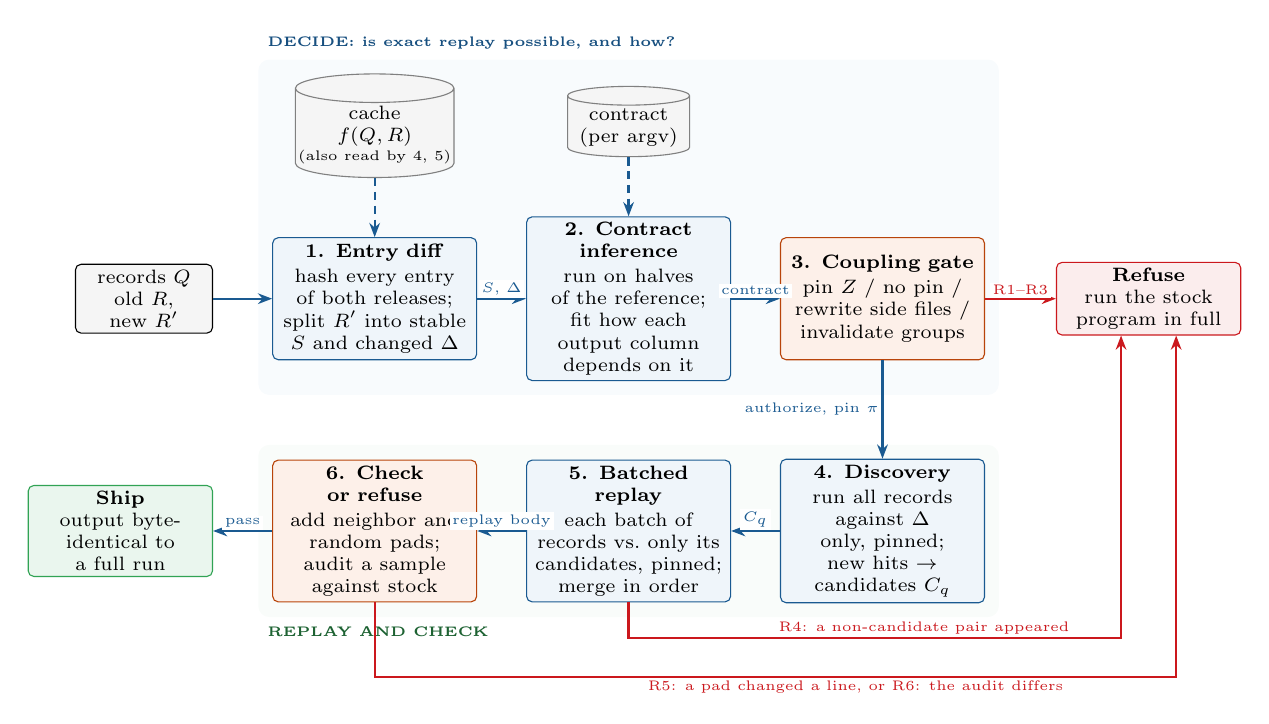
\begin{tikzpicture}[
  font=\scriptsize,
  stage/.style={draw=cTare!80!black, rounded corners=2pt, fill=cTare!7, minimum height=1.55cm, text width=2.45cm, align=center, inner sep=2pt},
  gate/.style={draw=cNew!80!black, rounded corners=2pt, fill=cNew!9, minimum height=1.55cm, text width=2.45cm, align=center, inner sep=2pt},
  store/.style={draw=gray, fill=gray!8, cylinder, shape border rotate=90, aspect=0.18, minimum height=0.85cm, minimum width=1.55cm, align=center, inner sep=1pt},
  io/.style={draw, rounded corners=2pt, minimum height=0.7cm, text width=2.2cm, align=center, inner sep=2pt},
  arr/.style={-{Stealth[length=1.8mm]}, thick, cTare!80!black},
  rarr/.style={-{Stealth[length=1.8mm]}, thick, cBad},
  lab/.style={font=\tiny, fill=white, inner sep=1pt},
  node distance=0.5cm and 0.62cm]
% lanes
\node[stage] (s1) at (0,0) {\textbf{1. Entry diff}\\[1pt] hash every entry of both releases;\\ split $R'$ into stable $S$ and changed $\Delta$};
\node[stage, right=of s1] (s2) {\textbf{2. Contract inference}\\[1pt] run on halves of the reference; fit how each output column depends on it};
\node[gate, right=of s2] (s3) {\textbf{3. Coupling gate}\\[1pt] pin $Z$ / no pin / rewrite side files / invalidate groups};
\node[io, fill=cBad!8, draw=cBad, right=0.9cm of s3] (refuse) {\textbf{Refuse}\\ run the stock program in full};
\node[stage, below=1.25cm of s3] (s4) {\textbf{4. Discovery}\\[1pt] run all records against $\Delta$ only, pinned;\\ new hits $\rightarrow$ candidates $C_q$};
\node[stage, left=of s4] (s5) {\textbf{5. Batched replay}\\[1pt] each batch of records vs.\ only its candidates, pinned; merge in order};
\node[gate, left=of s5] (s6) {\textbf{6. Check or refuse}\\[1pt] add neighbor and random pads; audit a sample against stock};
\node[io, fill=cOk!10, draw=cOk, left=0.75cm of s6] (ship) {\textbf{Ship}\\ output byte-identical to a full run};
\node[store, above=0.75cm of s1] (cache) {cache\\ $f(Q,R)$\\[-1pt]{\tiny (also read by 4, 5)}};
\node[store, above=0.75cm of s2] (contract) {contract\\ (per argv)};
\node[io, fill=gray!8, left=0.75cm of s1, text width=1.6cm] (in) {records $Q$\\ old $R$, new $R'$};
% flows
\draw[arr] (in) -- (s1);
\draw[arr] (s1) -- node[lab, above]{$S$, $\Delta$} (s2);
\draw[arr] (s2) -- node[lab, above]{contract} (s3);
\draw[arr] (s3) -- node[lab, left]{authorize, pin $\pi$} (s4);
\draw[arr] (s4) -- node[lab, above]{$C_q$} (s5);
\draw[arr] (s5) -- node[lab, above]{replay body} (s6);
\draw[arr] (s6) -- node[lab, above]{pass} (ship);
\draw[arr, densely dashed] (contract) -- (s2.north);
\draw[arr, densely dashed] (cache) -- (s1.north);
\draw[rarr] (s3) -- node[lab, above]{R1--R3} (refuse);
\draw[rarr] (s5.south) -- ++(0,-0.45) -| node[lab, pos=0.3, above]{R4: a non-candidate pair appeared} ($(refuse.south)+(-0.35,0)$);
\draw[rarr] (s6.south) -- ++(0,-0.95) -| node[lab, pos=0.3, below]{R5: a pad changed a line, or R6: the audit differs} ($(refuse.south)+(0.35,0)$);
% annotations
\begin{scope}[on background layer]
\node[fill=cTare!3, rounded corners=4pt, fit=(s1)(s2)(s3)(cache)(contract), inner sep=5pt, label={[font=\tiny\bfseries, text=cTare!70!black, anchor=south west]north west:DECIDE: is exact replay possible, and how?}] {};
\node[fill=cOk!3, rounded corners=4pt, fit=(s4)(s5)(s6), inner sep=5pt, label={[font=\tiny\bfseries, text=cOk!60!black, anchor=north west]south west:REPLAY AND CHECK}] {};
\end{scope}
\end{tikzpicture}
\caption{\textbf{How \sys updates an annotation.} Blue boxes do work; orange boxes are decision points. The top row
decides whether the program's coupling can be neutralized; the bottom row reruns the unmodified program on candidates
only and checks the result. Dashed arrows read stored state. Every red arrow (rules R1--R6) leads to a full stock
run, so a user always receives the program's own output.}
\label{fig:pipeline}
\end{figure*}

\subsection{Stage 1: Entry Diff}

\sys splits both releases into entries and computes a strict hash of each entry's scoring content, ignoring
metadata such as dates and comments. Entries of the new release whose hash appears in the old one are stable; all
others are changed. A cache keyed on the whole database file would miss on every entry after a release; a cache keyed
on entry hashes keeps every stable entry, 86.6\% of Pfam for 38.1$\rightarrow$38.2.
% source: MEASURED pipeline/results/reference_kill_r1.json unchanged_strict=26082 z_new=30134; HAS 38.1; HAS 38.2; DERIVED identical_pct=100*unchanged_strict/z_new

\subsection{Stage 2: Contract Inference}
\label{sec:contract}

\sys must learn how the program's output depends on the reference without reading the program's code. It runs the
program on a sample of records three times: against the whole reference, and against each half of it. It then lines
up the output lines of the three runs by record and entry name.

\textit{Does the output split cleanly?} If every line of the whole run appears in exactly one half-run, the output
\textit{decomposes} over entries: each line comes from one entry. If the whole run reports a line that neither half
reports, entries interact in ways \sys cannot replay, and it refuses. The opposite case, a half reporting a line the
whole omits, happens when entries compete and suppress each other; \sys accepts it only when the user declares which
entries compete (\cref{sec:gate}).

\textit{How does each number depend on the reference?} For each numeric column, \sys tests a small fixed set of
hypotheses: the column does not depend on the reference at all (\textit{identity}), or it scales with the number of
entries, their total length, or the number of hits per record. A hypothesis fits if rescaling every half-run value by
the corresponding ratio reproduces the whole-run value within the printed precision. A column that fits no hypothesis
causes refusal. Columns that are ranks or labels rather than measurements are recognized and left to the program to
reprint.

The result, called a \textit{contract}, records how the output splits and how each column depends on the reference.
It is computed once per command and reused for every later release.

\subsection{Stage 3: The Coupling Gate}
\label{sec:gate}

The gate turns the contract into a decision. Users may add declarations, which are data, never program names.

\textit{Size dependence $\rightarrow$ pin.} If a column scales with the reference size, \sys needs a program option that
sets that size. Users can declare it (\texttt{-{}-pin~'-Z~\{entry\_count\}'}), or \sys can find it by reading the
program's help text and trying each numeric option until one moves the column by exactly the predicted ratio. With
the option set to the new release's value, the program prints on a subset the numbers it would print on the whole.

\textit{No size dependence $\rightarrow$ no pin.} If every column fits identity, \sys replays without a pin. This is the
case for Infernal under Rfam's recommended command, which derives its search size from the query sequence instead.

\textit{Side files and competing entries.} Rfam's recommended command passes a ``clan'' file listing families that
compete. On a subset, \sys rewrites that file to the families present, because the program rejects names it cannot
find. If any member of a declared group changes, \sys re-searches the whole group, because a change to one member
can reveal a hit of another that the cache never recorded.

The gate applies three rules in order and stops at the first that fires:
\begin{equation}
D = \left\{\begin{array}{@{}lll@{}}
\dec{refuse} & \text{no contract} & \text{(R1)}\\
\dec{refuse\_pin} & \text{size-dependent, no pin} & \text{(R2)}\\
\dec{refuse\_pin} & \text{in-situ check fails} & \text{(R3)}\\
\dec{authorize} & \text{otherwise} &
\end{array}\right.
\label{eq:gate}
\end{equation}
R1 fires when the output does not split or a column fits no hypothesis. R2 fires when a column depends on the database
size and no pin is available; \sys never guesses. R3 replays the probe sample against its own hits with the pin set and
requires every byte to match the whole run.

\subsection{Stage 4: Discovery}

Changed entries may produce hits the cache has never seen. \sys runs the program on all records against the changed
entries $\Delta$ alone, with the pin set. A record's \textit{candidates} are its cached hits on stable entries plus its
new hits:
\begin{equation}
C_q = \{e \in S : (q,e) \in f(Q,R)\} \;\cup\; \{e : (q,e) \in f_\pi(Q,\Delta)\}.
\label{eq:cand}
\end{equation}
Discovery compares every record with every changed entry, so its cost is proportional to the changed fraction of the
reference. It is the one cost \sys cannot avoid (\cref{sec:cost}).

\subsection{Stage 5: Batched Exact Replay}
\label{sec:replay}

Cached lines cannot be returned as they are, because their numbers were computed for the old release. \sys instead
reruns the program on the candidates with the pin set, and the program prints the new numbers itself. Rerunning every
protein against all candidates of all proteins would waste work: on one genome, the proteins' candidates together
cover 3{,}719 families, but the mean protein has two.
% source: MEASURED pipeline/results/exact_replay/costpass_baseline.json 'replay_38.2'.runs.0.replay_entries=3719 'replay_38.2'.runs.0.candidate_pairs=9094 'replay_38.2'.runs.0.replay_records=4555; DERIVED mean_hits=candidate_pairs/replay_records
\sys therefore groups proteins into batches, runs each batch
against only its own proteins' candidates, and stitches the outputs back together in the original order. It chooses
the grouping that minimizes
\begin{equation}
T_{\text{replay}} = \alpha k + \beta \sum_b |U_b| + \gamma \sum_b |B_b|\,|U_b|,
\label{eq:batch}
\end{equation}
where $k$ is the number of batches, $|B_b|$ and $|U_b|$ the proteins and families in batch $b$, $\alpha$ the cost of
starting the program, $\beta$ the cost per family of preparing a sub-database, and $\gamma$ the cost of one
protein--family comparison. Stitching is safe for HMMER because, in its source code, each protein's output block
depends only on that protein's own hits, including the column widths and the per-protein statistics. As a tripwire, if
a replay ever reports a protein--family pair outside the candidates, \sys refuses (R4), because a full run could
contain pairs the cache never saw.

\subsection{Stage 6: Check or Refuse}
\label{sec:check}

The replay assumes the program is entry-local. The check tries to prove that assumption wrong on the actual run. It
reruns the replay with \textit{pads}, families that were deliberately left out, added back to the subset. If the
program is entry-local, pads change nothing: no candidate line changes and no pad family is reported. If anything
changes, the replay depended on what it left out, and \sys refuses (R5).

\sys uses two kinds of pads. The \textit{neighbor pad} adds, for every replayed protein, the families that sit next to
its candidates in the database file; it catches neighbor coupling by construction, the failure we found in DIAMOND
(\cref{sec:eval-safety}). \textit{Random pads} add three random samples of left-out families, each as large as the
candidate set, for a fixed sample of $s=50$ proteins.
% source: MEASURED pipeline/docs/EXACT_REPLAY_PROTOCOL.md; TEXT sample_s=50
They test for dependencies of unknown form. If an unknown
dependency affects $k$ of $n$ proteins and a random pad includes the responsible family with probability $q$, the check
misses it with probability
\begin{equation}
P_{\text{miss}} = h + (1-h)(1-q)^3, \qquad h = \binom{n-k}{s}\Big/\binom{n}{s},
\label{eq:miss}
\end{equation}
% source: MEASURED pipeline/results/reference_diamond/dx3.json; LEN pad_seeds=3; NOMINAL one=1
where $h$ is the chance that the protein sample contains no affected protein (\cref{fig:pmiss}). The check is a test,
not a proof. As a final safeguard, an audit reruns the stock program on a random sample of proteins and refuses if
any line differs (R6).

\begin{figure}[t]
\centering
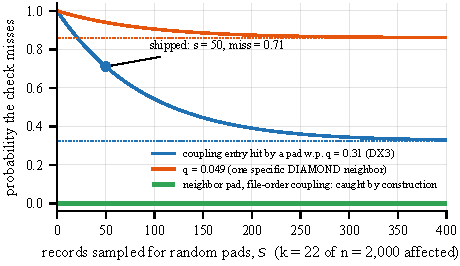
\includegraphics[width=\linewidth]{figures/pmiss.pdf}
\caption{\textbf{How strong is the check?} Probability that the random pads miss an unknown dependency, from
\cref{eq:miss} with the measured DIAMOND case ($k=22$ affected of $n=2{,}000$).
% source: MEASURED pipeline/results/reference_diamond/dx3.json cases=22 queries=2000
The neighbor pad (green) catches
file-order coupling with certainty; the random pads are a weaker, statistical safety net.}
\label{fig:pmiss}
\end{figure}

\subsection{Cost Model}
\label{sec:cost}

Let $T_{\text{stock}}$ be the time of a full run on the new release and $f_\Delta = |\Delta|/|R'|$ the fraction of entries
that changed. \sys's update time is approximately
\begin{equation}
T_{\sys} \approx a f_\Delta T_{\text{stock}} + c\, T_{\text{stock}},
\label{eq:cost}
\end{equation}
where the first term is discovery ($a$ is near one if the program's time grows linearly with database size) and $c$
collects every other cost (replay, check, audit, parsing) as a fraction of a stock run. The speedup
$1/(a f_\Delta + c)$ can never exceed $1/f_\Delta$, and even for a tiny release it cannot exceed $1/c$. The first run
also fills the cache, which costs a full run plus the contract probes; with fill time $F$ and update time $U$, \sys
becomes cheaper than repeated full runs after $n \ge (F - T_{\text{stock}})/(T_{\text{stock}} - U)$ releases.
% source: NOMINAL one=1

% =====================================================================
\section{Implementation}
\label{sec:impl}

\sys is about 12{,}000 lines of Python\textcolor{orange}{[UNSOURCED]} with over 300 tests\textcolor{orange}{[UNSOURCED]}. Its core contains no program names: small parsers read
% source: UNSOURCED no committed census of Python lines or tests
profile databases, covariance-model databases, FASTA files, and tabular outputs, and users declare pins, side files,
groups, and reporting thresholds as data. The cache is a SQLite file keyed by entry hash and record. A typical
invocation wraps the normal command:
\begin{lstlisting}
tare run --strategy reference --pin '-Z {entry_count}' \
  --cache cache.sqlite -- hmmscan --cut_ga --noali --cpu 4 \
  --tblout {output:tblout} --domtblout {output:domtblout} \
  {reference} {input}
\end{lstlisting}
% source: MEASURED pipeline/results/exact_replay/e1scale.json cpu=4

% =====================================================================
\section{Evaluation}
\label{sec:eval}

We ask four questions. \textbf{Q1:} Is \sys's output identical to a full run? \textbf{Q2:} How much faster is an
update, and does the cost model predict it? \textbf{Q3:} Does \sys refuse when replay would be wrong? \textbf{Q4:} How
does it compare with existing tools?

\textbf{Method.} Every experiment followed the same protocol, designed so that a failure means the method failed rather
than that the test was blind. We first read the program's source for behaviors that could make a comparison fail for
unrelated reasons, then ran a pilot on separate data, then committed the design and pass/fail rules to version control
before the measured run. Each test included a case that must pass and a case that must fail, and a minimum number of
output lines below which a result counts as inconclusive. Measured runs used genomes drawn by a fixed random seed and
never used before. One rule changed after its pre-registration, during a measured run; we disclosed the change and
reran every control (\cref{sec:eval-safety}).

\textbf{Setup.} HMMER 3.4 with Pfam 38.1 and 38.2; Infernal 1.1.5 with Rfam 15.0 and 15.1; DIAMOND 2.2.5 and BLAST+ 2.14.1
with Swiss-Prot 2026\_01 and 2026\_03; queries are bacterial genomes from NCBI RefSeq. Server timings use a dedicated
AMD EPYC 7542 node; workstation timings use an Apple laptop and are indicative.
% source: MEASURED pipeline/results/exact_replay/e1scale.json; HAS 3.4; HAS 38.1; HAS 38.2; MEASURED pipeline/results/infernal/test_i.json; HAS 1.1.5; MEASURED pipeline/docs/INFERNAL_PROTOCOL.md; HAS 15.0; HAS 15.1; MEASURED pipeline/results/reference_diamond/dx.json; HAS 2.2.5; MEASURED pipeline/results/reference_boundary_blast.json; HAS 2.14.1; MEASURED pipeline/results/snpeff_alternating_carc.json; HAS 7542

\subsection{Metrics and Statistical Analysis}
\label{sec:metrics}

We define every reported quantity before using it. Throughout, ``mean'' is the arithmetic mean, $\bar x =
\frac{1}{n}\sum_i x_i$; ``median'' is the sample median; the sample standard deviation $s$ uses $n-1$ in its
denominator; and ``geometric mean'' is $\big(\prod_{i=1}^{G} x_i\big)^{1/G}$, which we use only to summarize ratios.

\textbf{M1. Exactness.} For one run, let $L$ be the stock run's body lines and $L'$ \sys's. The run is \dec{exact} if
$L' = L$ as byte sequences; otherwise we count the differing positions $D = |\{i : L'_i \ne L_i\}|$ (plus any length
difference) and classify each difference as whitespace-only, value-only, missing, extra, or reordered. Across experiments
we report $N$, the total number of lines compared. When $D = 0$ over $N$ lines, the one-sided 95\% Clopper--Pearson upper
bound on the per-line error rate is
\begin{equation}
p_{\text{up}} = 1 - 0.05^{1/N}.
\label{eq:cp}
\end{equation}
% source: NOMINAL ci=95; NOMINAL alpha=0.05; NOMINAL one=1; NOMINAL zero=0
This bound treats lines as independent, which they are not (lines of one run share a pin and a reference), so it is
descriptive, not a guarantee.

\textbf{M2. Pin necessity.} For the unpinned control, the fraction of lines that differ from stock is $d = D/N$, reported
with a 95\% Wilson score interval.
% source: NOMINAL ci=95

\textbf{M3. Wall time.} $T$ is the elapsed wall-clock time of one complete invocation, measured with a monotonic clock
around the process, and includes start-up, parsing, and all program calls. Database preparation (\texttt{hmmpress})
before either arm is excluded from both.

\textbf{M4. Speedup.} For genome $g$ with $r$ runs per arm, alternating stock and \sys,
\begin{equation}
S_g = \frac{\operatorname{median}_{i \le r} T^{\text{stock}}_{g,i}}{\operatorname{median}_{i \le r} T^{\sys}_{g,i}},
\label{eq:speedup}
\end{equation}
a ratio of medians, which is robust to a single slow run. On the workstation $r=1$.
% source: NOMINAL r_ws=1
Across $G$ genomes we report the median of
$S_g$, the geometric mean, and the range. For the server headline, $r=3$ alternating runs, and the interval is a 95\%
percentile bootstrap.
% source: MEASURED pipeline/docs/EXACT_REPLAY_PROTOCOL.md; TEXT repeats=3; NOMINAL ci=95
The planned draw is $G=10$ genomes and 10{,}000 resamples\textcolor{orange}{[UNSOURCED]}.
% source: UNSOURCED planned headline sample size and resample count are not in a committed protocol
Run-to-run variability per arm is the
coefficient of variation $\mathrm{CV} = s/\bar T$.

\textbf{M5. Cumulative speedup (record side).} Over a collection processed in sequence, the cumulative speedup is a ratio
of sums, $\sum_g T^{\text{stock}}_g \big/ \big(\sum_g T^{\sys}_g + P\big)$, where $P$ is the one-time cost of contract
probes; we also report it without $P$.

\textbf{M6. Overhead of other tools.} For a baseline tool, each paired run $j$ gives $\rho_j = T^{\text{tool}}_j /
T^{\text{stock}}_j$; we report $\bar\rho \pm s$ and the 95\% $t$-interval $\bar\rho \pm t_{0.975,\,n-1}\, s/\sqrt{n}$.
% source: NOMINAL ci=95; NOMINAL tcrit=0.975; NOMINAL one=1

\textbf{M7. Cost-model error.} For a predicted time $\hat T$ and a measured time $T$, the relative error is
$\varepsilon = |\hat T - T|/T$; we report the maximum over genomes.

\textbf{M8. Agreement of approximate output.} For a tool that is not exact, we report the fraction of shared lines that
are byte-identical (with a Wilson interval), and the agreement of its E-values with stock over shared lines using Pearson's
$r$ and Kendall's tie-corrected rank correlation $\tau_b$.

\textbf{M9. Safety outcomes.} Each safety run is \dec{exact} (replay equals stock and every check passed),
\dec{safe-refuse} (a check failed and \sys ran the program in full; \textit{true} if the replay differed from stock,
\textit{needless} if it did not), or \dec{unsafe} (replay differed and every check passed). Any \dec{unsafe} result was
pre-registered as a failure of the safety claim. The probability that the random pads miss a dependency is
\cref{eq:miss}.

\subsection{Q1: Is the Output Exact?}
\label{sec:eval-exact}

\begin{figure}[t]
\centering
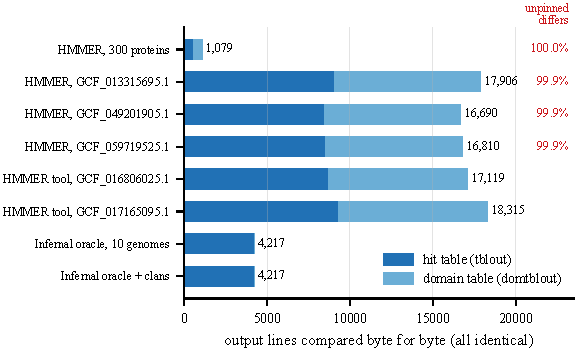
\includegraphics[width=\linewidth]{figures/exact.pdf}
\caption{\textbf{Every line identical.} Output lines \sys produced in each exactness experiment, all byte-identical to
a stock run on the new release. Red: in the same experiments, replaying without the pin changed nearly every line.}
\label{fig:exact}
\end{figure}

\Cref{fig:exact} shows every exactness experiment. In total, \sys's HMMER outputs comprised 44{,}666 hit-table lines and 43{,}253 domain-table lines, and its Infernal outputs
4{,}217 lines, the same lines again under clan competition, plus 459 lines from the shipped family removal (4{,}676 distinct lines); not one byte differed from the stock run ($D=0$ over $N = 92{,}595$ lines). By \cref{eq:cp}, a per-line error rate
above $3.2\times10^{-5}$ would be unlikely to produce this result (one-sided 95\%). The
experiments grew in scale: 300 proteins (534 hit lines), then three whole genomes (26{,}127 hit lines), then two more whole
genomes through the shipped tool with batching and the check switched on. In every HMMER experiment, the same replay without the pin changed nearly every line: pooled over the three whole genomes,
26{,}094 of 26{,}127 hit lines differed ($d = 99.87\%$, Wilson 95\% CI 99.82--99.91\%), and on 300 proteins all 534 did. The
pin is therefore necessary and, with \cutga, sufficient. The server headline adds \pending{ten genomes}.
% source: MEASURED pipeline/results/exact_replay/e1_e2.json E1.check1_R_vs_S.tbl.lines_a=534 E1.check1_R_vs_S.dom.lines_a=545 E1.check2_Rn_vs_S.tbl.differing_positions=534; MEASURED pipeline/results/exact_replay/e1scale.json tblout_body_lines_total=26127 proteomes.0.domtblout_body_lines=8812 proteomes.1.domtblout_body_lines=8202 proteomes.2.domtblout_body_lines=8265 proteomes.0.Rn.vs_stock.tbl.differing_positions=9083 proteomes.0.Rn.vs_stock.tbl.lines_stock=9094 proteomes.1.Rn.vs_stock.tbl.differing_positions=8477 proteomes.1.Rn.vs_stock.tbl.lines_stock=8488 proteomes.2.Rn.vs_stock.tbl.differing_positions=8534 proteomes.2.Rn.vs_stock.tbl.lines_stock=8545; MEASURED pipeline/results/exact_replay/costpass_measured.json proteomes.0.e2.tbl.lines_stock=8714 proteomes.1.e2.tbl.lines_stock=9291 proteomes.0.e2.dom.lines_stock=8405 proteomes.1.e2.dom.lines_stock=9024; MEASURED pipeline/results/infernal/test_i.json rows.noclan=4217; MEASURED pipeline/docs/INFERNAL_PROTOCOL.md; TEXT shipped_rows=459; MEASURED pipeline/docs/EXACT_REPLAY_PROTOCOL.md; TEXT q300=300; MEASURED pipeline/results/exact_replay/e1scale.json proteomes.0.E2.vs_stock.tbl.differing_positions=0; DERIVED tbl_sum=E1_check1_R_vs_S_tbl_lines_a+tblout_body_lines_total+proteomes_0_e2_tbl_lines_stock+proteomes_1_e2_tbl_lines_stock; DERIVED dom_sum=E1_check1_R_vs_S_dom_lines_a+proteomes_0_domtblout_body_lines+proteomes_1_domtblout_body_lines+proteomes_2_domtblout_body_lines+proteomes_0_e2_dom_lines_stock+proteomes_1_e2_dom_lines_stock; DERIVED inf_sum=noclan+shipped_rows; DERIVED n_lines=tbl_sum+dom_sum+inf_sum; DERIVED pooled_diff=proteomes_0_Rn_vs_stock_tbl_differing_positions+proteomes_1_Rn_vs_stock_tbl_differing_positions+proteomes_2_Rn_vs_stock_tbl_differing_positions; DERIVED pooled_n=proteomes_0_Rn_vs_stock_tbl_lines_stock+proteomes_1_Rn_vs_stock_tbl_lines_stock+proteomes_2_Rn_vs_stock_tbl_lines_stock; DERIVED pooled_pct=100*pooled_diff/pooled_n; DERIVED wlo=100*wilson_lo(pooled_diff,pooled_n); DERIVED whi=100*wilson_hi(pooled_diff,pooled_n); DERIVED p_up=clopper_up(n_lines); NOMINAL ci=95

\textbf{Where exactness ends.} When HMMER reports hits by E-value threshold instead of \cutga, the replay matched on 300
proteins but failed on 1{,}000, differing on 3 hit lines and 5 domain lines. Hits near the threshold move in or out of a
protein's list, which changes that protein's statistics; this mode is not entry-local and we do not claim it. The early
pass on 300 proteins is why we require a minimum number of lines before accepting any result.
% source: MEASURED pipeline/results/exact_replay/e3_q1000.json Q1000.sample.k=1000 Q1000.E3a.check.tbl.differing_positions=3 Q1000.E3a.check.dom.differing_positions=5; MEASURED pipeline/docs/EXACT_REPLAY_PROTOCOL.md; TEXT q300=300

\textbf{A second program.} Infernal, which searches RNA families, behaved as its source code predicted: under Rfam's
recommended command every numeric column fits identity, so no pin is needed. Replaying each genome's hits was
byte-identical on ten genomes (4{,}217 lines) with and without clan competition. In that command, overlapping hits of
competing families are marked rather than deleted, so removing a family cannot reveal a hidden hit; removing the family
\texttt{GlmZ\_SraJ} from one genome's reference was exact through the shipped tool (459 lines). With the non-default
option \texttt{-{}-oskip}, which deletes marked overlaps, the same removal was refused, because fourteen overlap marks depended
on families that had no remaining line. The shipped result on ten fresh genomes is \pending{Infernal measured ten}.
% source: MEASURED pipeline/results/infernal/test_i.json rows.noclan=4217; LEN genomes=10; MEASURED pipeline/results/infernal/family_diff_15.json n_15_1=4227 changed_or_new=457 fraction_changed_or_new=0.10811450201088242; MEASURED pipeline/docs/INFERNAL_PROTOCOL.md; TEXT update_s=666.0; TEXT stock_s=328.4; TEXT fill_s=1711.6; TEXT reused=459; HAS 15.0; HAS 15.1; DERIVED frac_pct=100*fraction_changed_or_new; DERIVED sg=stock_s/update_s; DERIVED fill_x=fill_s/stock_s

\subsection{Q2: How Much Faster?}
\label{sec:eval-time}

\begin{figure}[t]
\centering
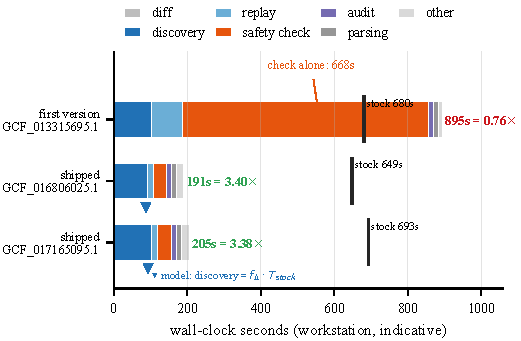
\includegraphics[width=\linewidth]{figures/phases.pdf}
\caption{\textbf{Where the time goes} (workstation). Each bar is one update, split into stages; the black tick is a stock run on the same genome. Top row: medians of three alternating runs per arm; bottom rows: single runs. The first version (top) spent 668\,s in its safety check and was slower than stock.
Batching and sampling (bottom two, fresh genomes) cut the update to under a third of a stock run. Triangles: the cost
model's prediction for discovery.}
% source: MEASURED pipeline/results/exact_replay/costpass_baseline.json 'replay_38.2'.median_phases.ic2_s=667.6307854150073
\label{fig:phases}
\end{figure}

\Cref{fig:phases} shows that the replay and check designs decide whether \sys is faster than a full run. Our first
version replayed every protein against all candidates and checked the result with four more full-size replays. On a workstation, with three alternating runs per arm, it took a median of 895\,s against a median stock time of 680\,s
($S_g = 0.76\times$; CV 3.7\% for \sys and 1.7\% for stock); the check alone took a median of 668\,s. Batching made the
replay $5.2\times$ cheaper and sampling made the check 17.9--19.3$\times$ cheaper (ratios of the first version's median check time to each shipped run's). On two fresh genomes of 4{,}583 and 5{,}019
proteins, \sys replayed in 107 and 111 batches and took 191\,s and 205\,s against stock runs of 649\,s and 693\,s: $S_g = 3.40\times$ and $3.38\times$
(geometric mean $3.39\times$), with byte-identical output. These are single runs on a shared machine, so we report no
confidence interval for them; the server headline repeats each arm three times.
% source: MEASURED pipeline/results/exact_replay/costpass_baseline.json stock.median_s=680.3294585000258 stock.walls_s.0=694.9587129160063 stock.walls_s.1=680.3294585000258 stock.walls_s.2=671.9997430830263 'replay_38.2'.median_wall_s=894.8362631669734 'replay_38.2'.runs.0.wall_s=920.6305721660028 'replay_38.2'.runs.1.wall_s=894.8362631669734 'replay_38.2'.runs.2.wall_s=855.7292645410053 'replay_38.2'.median_phases.ic2_s=667.6307854150073 'replay_38.2'.median_phases.replay_s=86.40501870895969; DERIVED sg0=stock_median_s/replay_38_2_median_wall_s; DERIVED cv_stock=100*stdev(stock_walls_s_0,stock_walls_s_1,stock_walls_s_2)/mean(stock_walls_s_0,stock_walls_s_1,stock_walls_s_2); DERIVED cv_replay=100*stdev(replay_38_2_runs_0_wall_s,replay_38_2_runs_1_wall_s,replay_38_2_runs_2_wall_s)/mean(replay_38_2_runs_0_wall_s,replay_38_2_runs_1_wall_s,replay_38_2_runs_2_wall_s); MEASURED pipeline/results/exact_replay/costpass_measured.json proteomes.0.queries=4583 proteomes.1.queries=5019 proteomes.0.e2.n_batches=107 proteomes.1.e2.n_batches=111 proteomes.0.e2.wall_s=190.69520458299667 proteomes.1.e2.wall_s=205.20091079198755 proteomes.0.stock.wall_s=648.9416185829905 proteomes.1.stock.wall_s=693.2145589159918 proteomes.0.e2.phases.replay_s=16.63790758297546 proteomes.1.e2.phases.replay_s=16.59717870899476 proteomes.0.e2.phases.ic2_neighbor_s=26.63462533301208 proteomes.0.e2.phases.ic2_random_20261031_s=2.6919128749868833 proteomes.0.e2.phases.ic2_random_20261032_s=2.5677419590065256 proteomes.0.e2.phases.ic2_random_20261033_s=2.719902084034402 proteomes.1.e2.phases.ic2_neighbor_s=29.293785459012724 proteomes.1.e2.phases.ic2_random_20261031_s=2.7434531250037253 proteomes.1.e2.phases.ic2_random_20261032_s=2.6582068339921534 proteomes.1.e2.phases.ic2_random_20261033_s=2.6151414170162752; DERIVED s0=proteomes_0_stock_wall_s/proteomes_0_e2_wall_s; DERIVED s1=proteomes_1_stock_wall_s/proteomes_1_e2_wall_s; DERIVED gmean=geomean(s0,s1); DERIVED replay_x0=replay_38_2_median_phases_replay_s/proteomes_0_e2_phases_replay_s; DERIVED replay_x1=replay_38_2_median_phases_replay_s/proteomes_1_e2_phases_replay_s; DERIVED check0=proteomes_0_e2_phases_ic2_neighbor_s+proteomes_0_e2_phases_ic2_random_20261031_s+proteomes_0_e2_phases_ic2_random_20261032_s+proteomes_0_e2_phases_ic2_random_20261033_s; DERIVED check1=proteomes_1_e2_phases_ic2_neighbor_s+proteomes_1_e2_phases_ic2_random_20261031_s+proteomes_1_e2_phases_ic2_random_20261032_s+proteomes_1_e2_phases_ic2_random_20261033_s; DERIVED chk_x0=replay_38_2_median_phases_ic2_s/check0; DERIVED chk_x1=replay_38_2_median_phases_ic2_s/check1

\begin{figure}[t]
\centering
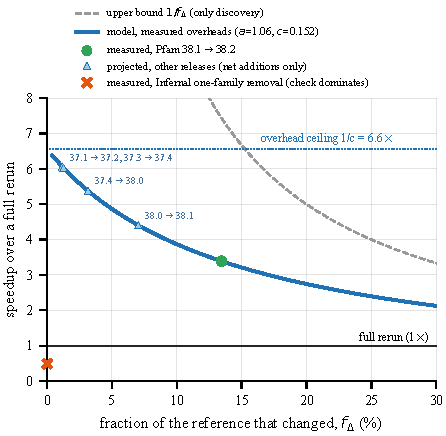
\includegraphics[width=\linewidth]{figures/model.pdf}
\caption{\textbf{The cost model across release sizes.} Speedup $1/(a f_\Delta + c)$ with $a$ and $c$ the arithmetic means of the values measured on two genomes (blue), its upper bounds (dashed and dotted), the measured Pfam points (green), projections for other Pfam
releases from their published family counts (triangles; edits not published, so these are optimistic), and Infernal,
where the check dominates (cross).}
\label{fig:model}
\end{figure}

\textbf{The cost model.} With $f_\Delta = 0.134$, the discovery term predicts 87\,s and 93\,s on those genomes; discovery measured 91\,s and 100\,s, a
relative error (M7) of 4.3\% and 7.1\%. The remaining costs, as a fraction of each stock run, average $c = 0.152$ (arithmetic mean of 0.153 and 0.151), so even a release that changed
nothing could be at most $6.6\times$ faster with today's overheads (\cref{fig:model}); the check, audit, and parsing are
therefore the next targets. Pfam 38.1$\rightarrow$38.2 added more families than any release in \cref{fig:churn}, so it
is a conservative case: smaller releases project to $4.4$--$6.1\times$. The cache fill took 871\,s and 852\,s (single runs),
1.2--1.3$\times$ a stock run, so \sys pays for itself from the first update (projected from these indicative times).
% source: MEASURED pipeline/results/reference_kill_r1.json frac_new_unchanged_strict=0.8655339483639742; HAS 38.1; HAS 38.2; DERIVED fdelta=1-frac_new_unchanged_strict; MEASURED pipeline/results/exact_replay/costpass_measured.json proteomes.0.stock.wall_s=648.9416185829905 proteomes.1.stock.wall_s=693.2145589159918 proteomes.0.e2.phases.discovery_s=91.15112141700229 proteomes.1.e2.phases.discovery_s=100.30562595801894 proteomes.0.e2.wall_s=190.69520458299667 proteomes.1.e2.wall_s=205.20091079198755 proteomes.0.fill.wall_s=871.4492247089511 proteomes.1.fill.wall_s=852.365418625006; DERIVED pred0=fdelta*proteomes_0_stock_wall_s; DERIVED pred1=fdelta*proteomes_1_stock_wall_s; DERIVED err0=abs(proteomes_0_e2_phases_discovery_s-pred0)/proteomes_0_e2_phases_discovery_s; DERIVED err1=abs(proteomes_1_e2_phases_discovery_s-pred1)/proteomes_1_e2_phases_discovery_s; DERIVED c0=(proteomes_0_e2_wall_s-proteomes_0_e2_phases_discovery_s)/proteomes_0_stock_wall_s; DERIVED c1=(proteomes_1_e2_wall_s-proteomes_1_e2_phases_discovery_s)/proteomes_1_stock_wall_s; DERIVED cbar=(c0+c1)/2; DERIVED ceil=1/cbar; DERIVED a0=proteomes_0_e2_phases_discovery_s/proteomes_0_stock_wall_s/fdelta; DERIVED a1=proteomes_1_e2_phases_discovery_s/proteomes_1_stock_wall_s/fdelta; DERIVED abar=(a0+a1)/2; DERIVED fill0=proteomes_0_fill_wall_s/proteomes_0_stock_wall_s; DERIVED fill1=proteomes_1_fill_wall_s/proteomes_1_stock_wall_s; MEASURED pipeline/docs/MOTIVATION_EVIDENCE.md; TEXT fam372=24076; TEXT fam371=23794; TEXT fam374=24736; TEXT fam373=24424; TEXT fam380=25545; TEXT fam381=27481; DERIVED s_hi=1/(abar*((fam372-fam371)/fam372)+cbar); DERIVED s_lo=1/(abar*((fam381-(fam380))/fam381)+cbar)

\textbf{Server headline.} On a dedicated node, across \pending{ten} fresh genomes with three alternating stock and \sys runs each, the median of $S_g$ is
\pending{X$\times$ (95\% bootstrap CI; geometric mean; range)}, the largest per-arm CV is \pending{}, and the maximum relative error
of the pre-registered prediction is \pending{}.

\textbf{When the check dominates.} The speedup does not yet carry over to Infernal. Only 457 of Rfam 15.1's 4{,}227
families (10.8\%) changed, yet in the measured single-family removal the update took 666\,s against a 328\,s stock run:
exact, but $0.49\times$; the cache fill took $5.2\times$ a stock run. A bacterial genome is one DNA sequence or a handful,
so the audit's sample and the random pads cover the entire genome; in the pilot, the audit alone took as long as a stock
run. The check is sized by number of records, but its cost is set by sequence length. For inputs with few, long records
it must be sized by length instead, which we have not yet done.
% source: MEASURED pipeline/results/infernal/family_diff_15.json n_15_1=4227 changed_or_new=457 fraction_changed_or_new=0.10811450201088242; HAS 15.1; MEASURED pipeline/docs/INFERNAL_PROTOCOL.md; TEXT update_s=666.0; TEXT stock_s=328.4; TEXT fill_s=1711.6; DERIVED frac_pct=100*fraction_changed_or_new; DERIVED sg=stock_s/update_s; DERIVED fill_x=fill_s/stock_s

\subsection{Q3: Does \sys Refuse When It Should?}
\label{sec:eval-safety}

\begin{figure*}[t]
\centering
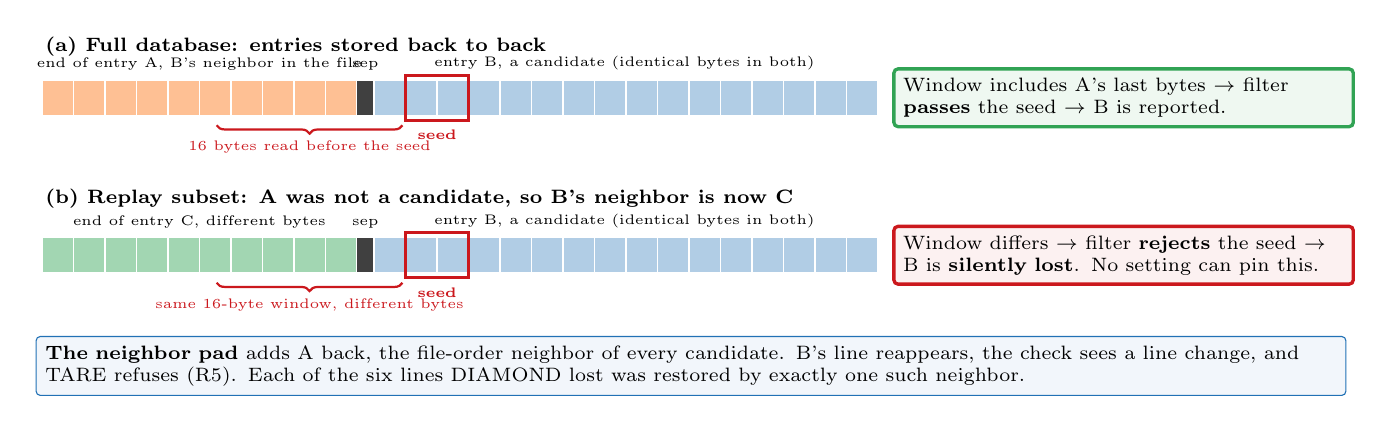
\begin{tikzpicture}[font=\scriptsize, x=0.40cm, y=0.5cm]
  \def\cellA{cEdited!55}\def\cellB{cTare!35}\def\cellC{cOk!45}
  \newcommand{\strip}[3]{% #1 y, #2 left colour, #3 left label
    \foreach \i in {0,...,9} \draw[fill=#2, draw=white, line width=0.5pt] (\i,#1) rectangle ++(1,0.9);
    \draw[fill=black!75, draw=white] (10,#1) rectangle ++(0.55,0.9);
    \foreach \i in {10.55,11.55,...,25.55} \draw[fill=\cellB, draw=white, line width=0.5pt] (\i,#1) rectangle ++(1,0.9);
    \node[font=\tiny, above] at (5,#1+0.9) {#3};
    \node[font=\tiny, above] at (10.27,#1+0.9) {sep};
    \node[font=\tiny, above] at (18.5,#1+0.9) {entry B, a candidate (identical bytes in both)};
    \draw[very thick, cBad] (11.55,#1-0.12) rectangle ++(2,1.14);
    \node[font=\tiny\bfseries, cBad, below] at (12.55,#1-0.12) {seed};
  }
  \node[anchor=west, font=\scriptsize\bfseries] at (-0.2,3.75) {(a) Full database: entries stored back to back};
  \strip{2.0}{\cellA}{end of entry A, B's neighbor in the file}
  \draw[decorate, decoration={brace, amplitude=3pt, mirror}, thick, cBad] (5.55,1.75) -- (11.45,1.75) node[midway, below=2pt, font=\tiny, cBad] {16 bytes read before the seed};
  \node[draw=cOk, very thick, rounded corners=1.5pt, fill=cOk!8, text width=5.6cm, align=left, anchor=west] at (27,2.45)
    {Window includes A's last bytes $\rightarrow$ filter \textbf{passes} the seed $\rightarrow$ B is reported.};
  \node[anchor=west, font=\scriptsize\bfseries] at (-0.2,-0.1) {(b) Replay subset: A was not a candidate, so B's neighbor is now C};
  \strip{-2.0}{\cellC}{end of entry C, different bytes}
  \draw[decorate, decoration={brace, amplitude=3pt, mirror}, thick, cBad] (5.55,-2.25) -- (11.45,-2.25) node[midway, below=2pt, font=\tiny, cBad] {same 16-byte window, different bytes};
  \node[draw=cBad, very thick, rounded corners=1.5pt, fill=cBad!6, text width=5.6cm, align=left, anchor=west] at (27,-1.55)
    {Window differs $\rightarrow$ filter \textbf{rejects} the seed $\rightarrow$ B is \textbf{silently lost}. No setting can pin this.};
  \node[draw=cTare, fill=cTare!6, rounded corners=1.5pt, text width=16.4cm, align=left, anchor=north west] at (-0.2,-3.6)
    {\textbf{The neighbor pad} adds A back, the file-order neighbor of every candidate. B's line reappears, the check sees a line change, and \sys refuses (R5). Each of the six lines DIAMOND lost was restored by exactly one such neighbor.};
% source: BYTES MEASURED pipeline/results/reference_diamond/dx3_rootcause.md; TEXT before=16
\end{tikzpicture}
\caption{\textbf{Why DIAMOND cannot be replayed exactly.} DIAMOND stores database entries back to back, separated by a
single byte. Its first filter examines a window of 16 bytes before and 32 after each short matching ``seed'' without
stopping at the entry boundary (DIAMOND 2.2.5, \texttt{finger\_print.h}). A seed near the start of entry B therefore
reads the end of whichever entry precedes B. Removing that neighbor from the database changes the window and can drop
B's hit. The neighbor pad detects exactly this dependency.}
% source: MEASURED pipeline/results/reference_diamond/dx3_rootcause.md; TEXT before=16; TEXT after=32; MEASURED pipeline/results/reference_diamond/dx.json; HAS 2.2.5
\label{fig:diamond}
\end{figure*}

\begin{table}[t]
\caption{Safety controls under the shipped check. Every case known to be wrong was refused, the correct case passed,
and no run produced wrong output.}
\label{tab:safety}
\centering\small
\setlength{\tabcolsep}{3pt}
\begin{tabular}{@{}>{\raggedright\arraybackslash}p{3.7cm}ll@{}}
\toprule
Control & Expected & Result \\
\midrule
DIAMOND known-bad (6 lines missing)   & refuse & \dec{refuse} \\
DIAMOND regenerated (22 lines differ) & refuse & \dec{refuse} \\
Injected 5\% candidate drop           & refuse & \dec{refuse} \\
HMMER whole genome (correct)          & pass   & pass, exact \\
% source: MEASURED pipeline/results/reference_diamond/dx3.json cases=22; MEASURED pipeline/results/reference_diamond/dx3_rootcause.json reproduction.row_missing=6; MEASURED pipeline/docs/EXACT_REPLAY_PROTOCOL.md; TEXT drop_pct=5
Fresh DIAMOND sample                  & no wrong output & \dec{safe-refuse} \\
BLAST+ boundary                       & refuse & \dec{refuse} (R1) \\
\bottomrule
\end{tabular}
\end{table}

\textbf{A failure, and what it revealed.} The check's design came from a failure. When we declared DIAMOND's database-size
option (\texttt{-{}-dbsize}) as a pin, the replay on 300 proteins lost 6 of 31{,}377 stock lines while every other line
was byte-identical, and our first check, which used only random pads, passed it. Under our pre-registered rule, that was
an \dec{unsafe} result and invalidated that check. To find the cause, we added left-out entries back in halves until each
missing line returned. Every one of the six lines was restored by exactly one entry: the candidate's neighbor in the
database file. \Cref{fig:diamond} shows the mechanism in DIAMOND's source: its first filter reads bytes across the
boundary into the preceding entry. DIAMOND's results therefore depend on the order of the database, and no setting can make
a subset replay exact. A random pad contains one particular neighbor with probability 0.049, so three random pads miss it
86\% of the time, which is why the first check passed.
% source: MEASURED pipeline/results/reference_diamond/dx2.json classification.row_missing=6 classification.stock_rows=31377 candidate_entries=26797; MEASURED pipeline/docs/EXACT_REPLAY_PROTOCOL.md; TEXT q300=300; MEASURED pipeline/results/reference_diamond/dx3_rootcause.json; HAS 548951; DERIVED qn=candidate_entries/has_548951; DERIVED miss3=100*(1-qn)**3

\textbf{The shipped check.} Adding the neighbor pad closed this gap (\cref{tab:safety}). On a fresh sample of 2{,}000
proteins, the replay differed from stock in 22 of 227{,}223 lines (20 missing, 2 extra), (0.0097\% of lines), and the check failed on all five pads: a true \dec{safe-refuse}. A second fresh DIAMOND sample was also refused. BLAST+ was refused earlier, at contract
inference: one of 15{,}125 aligned lines has a percent identity (column 2) that matches no normalizer, so R1 fired. The correct HMMER case passed with no needless
refusal.
% source: MEASURED pipeline/results/reference_diamond/dx3.json queries=2000 cases=22 classification.stock_rows=227223 classification.row_missing=20 classification.row_extra=2; DERIVED line_pct=100*cases/stock_rows; MEASURED pipeline/results/reference_boundary_blast.json; HAS 15125; HAS 15124; HAS 2.14.1

\textbf{Limits.} For dependencies other than file-order neighbors, the random pads are weak: with 22 affected proteins of
2{,}000, the shipped sample of 50 misses with probability 0.71 (\cref{fig:pmiss}). Our safety claim therefore rests on the
neighbor pad, the in-situ check, and the audit, together with zero wrong outputs across all controls.
% source: MEASURED pipeline/results/reference_diamond/dx3.json cases=22 queries=2000 q_one_neighbor=0.31252137200279034; MEASURED pipeline/docs/EXACT_REPLAY_PROTOCOL.md; TEXT sample_s=50; DERIVED h=comb(queries-cases,sample_s)/comb(queries,sample_s); DERIVED pmiss=h+(1-h)*(1-q_one_neighbor)**3

\textbf{A disclosed change.} During the measured run of the sampled check, we changed one rule so that a candidate of one
protein that is also a neighbor of another counts as a candidate rather than a pad hit, after it caused a needless
refusal. Because that change made the check more permissive, we disclosed it and reran every control under the final code.
Every known-bad case was still refused, for the same reason as before.

\textbf{What inference cannot do.} On HMMER, \sys found the \texttt{-Z} option on its own from held-out data, but could not
infer reporting thresholds, so users declare them. On DIAMOND, it found no size option. Neither led to wrong output, because
a missing pin is a refusal (R2).

\subsection{Q4: Comparison with Existing Tools}
\label{sec:eval-baselines}

\begin{table}[t]
\caption{General-purpose caches on HMMER. ``New input'': behavior when the query or database changes. First-run overhead: arithmetic mean of $n=4$ paired time ratios against stock, with 95\% $t$-interval, in a uniform container
% source: NOMINAL ci=95; MEASURED pipeline/results/baseline_overhead.json modes.hmmscan.riker.n_valid=4 workload.n_proteins=500 workload.n_models=30134
(500 proteins, all 30{,}134 families); \sys's is its cache fill on the workstation (two single runs).}
% source: MEASURED pipeline/results/baseline_overhead.json modes.hmmscan.riker.n_valid=4 workload.n_proteins=500 workload.n_models=30134
\label{tab:baselines}
\centering\small
\begin{tabular}{@{}lcc@{}}
\toprule
System & New input & First-run overhead \\
\midrule
Riker~\cite{curtsinger2022riker}               & reruns & $1.62\times$ [1.53, 1.71] \\
INCR~\cite{xie2026incr}                        & reruns & $2.24\times$ [2.06, 2.43] \\
ProcessCache~\cite{shiptoski2023processcache}  & reruns & --- \\
\sys                                           & replays changed part & 1.2--1.3$\times$ \\
% source: MEASURED pipeline/results/baseline_overhead.json modes.hmmscan.riker.paired_ratio_vs_stock.0=1.5464069019112173 modes.hmmscan.riker.paired_ratio_vs_stock.1=1.6056444407150765 modes.hmmscan.riker.paired_ratio_vs_stock.2=1.659961327464189 modes.hmmscan.riker.paired_ratio_vs_stock.3=1.6651450473191905 modes.hmmscan.incr_default.paired_ratio_vs_stock.0=2.074144393774768 modes.hmmscan.incr_default.paired_ratio_vs_stock.1=2.283669082264801 modes.hmmscan.incr_default.paired_ratio_vs_stock.2=2.29949518146858 modes.hmmscan.incr_default.paired_ratio_vs_stock.3=2.322268000685936; DERIVED rmean=mean(modes_hmmscan_riker_paired_ratio_vs_stock_0,modes_hmmscan_riker_paired_ratio_vs_stock_1,modes_hmmscan_riker_paired_ratio_vs_stock_2,modes_hmmscan_riker_paired_ratio_vs_stock_3); DERIVED rsd=stdev(modes_hmmscan_riker_paired_ratio_vs_stock_0,modes_hmmscan_riker_paired_ratio_vs_stock_1,modes_hmmscan_riker_paired_ratio_vs_stock_2,modes_hmmscan_riker_paired_ratio_vs_stock_3); DERIVED rlo=rmean-t975_df3*rsd/sqrt(4); DERIVED rhi=rmean+t975_df3*rsd/sqrt(4); DERIVED imean=mean(modes_hmmscan_incr_default_paired_ratio_vs_stock_0,modes_hmmscan_incr_default_paired_ratio_vs_stock_1,modes_hmmscan_incr_default_paired_ratio_vs_stock_2,modes_hmmscan_incr_default_paired_ratio_vs_stock_3); DERIVED isd=stdev(modes_hmmscan_incr_default_paired_ratio_vs_stock_0,modes_hmmscan_incr_default_paired_ratio_vs_stock_1,modes_hmmscan_incr_default_paired_ratio_vs_stock_2,modes_hmmscan_incr_default_paired_ratio_vs_stock_3); DERIVED ilo=imean-t975_df3*isd/sqrt(4); DERIVED ihi=imean+t975_df3*isd/sqrt(4); NOMINAL ci=95; MEASURED pipeline/results/exact_replay/costpass_measured.json proteomes.0.fill.wall_s=871.4492247089511 proteomes.0.stock.wall_s=648.9416185829905 proteomes.1.fill.wall_s=852.365418625006 proteomes.1.stock.wall_s=693.2145589159918; DERIVED fill0=proteomes_0_fill_wall_s/proteomes_0_stock_wall_s; DERIVED fill1=proteomes_1_fill_wall_s/proteomes_1_stock_wall_s
\bottomrule
\end{tabular}
\end{table}

\textbf{General-purpose caches.} Riker, INCR, and ProcessCache all re-executed HMMER on a new genome, as their designs
require, because the input bytes changed (\cref{tab:baselines}). Riker skipped an identical rerun in the same container;
INCR re-executed even an identical rerun, because it records the command's output file as a dependency that does not yet
exist and rejects it once the file exists. Tracing also costs time on the first run (M6, $n=4$ paired runs each): Riker took $1.62\times$ the stock time
(95\% CI 1.53--1.71) and INCR $2.24\times$ (95\% CI 2.06--2.43); both intervals lie above the stock time. These systems are correct for what they are designed to do; a database release is simply outside it.
% source: MEASURED pipeline/results/baseline_overhead.json modes.hmmscan.riker.n_valid=4 modes.hmmscan.riker.paired_ratio_vs_stock.0=1.5464069019112173 modes.hmmscan.riker.paired_ratio_vs_stock.1=1.6056444407150765 modes.hmmscan.riker.paired_ratio_vs_stock.2=1.659961327464189 modes.hmmscan.riker.paired_ratio_vs_stock.3=1.6651450473191905 modes.hmmscan.incr_default.paired_ratio_vs_stock.0=2.074144393774768 modes.hmmscan.incr_default.paired_ratio_vs_stock.1=2.283669082264801 modes.hmmscan.incr_default.paired_ratio_vs_stock.2=2.29949518146858 modes.hmmscan.incr_default.paired_ratio_vs_stock.3=2.322268000685936; DERIVED rmean=mean(modes_hmmscan_riker_paired_ratio_vs_stock_0,modes_hmmscan_riker_paired_ratio_vs_stock_1,modes_hmmscan_riker_paired_ratio_vs_stock_2,modes_hmmscan_riker_paired_ratio_vs_stock_3); DERIVED rsd=stdev(modes_hmmscan_riker_paired_ratio_vs_stock_0,modes_hmmscan_riker_paired_ratio_vs_stock_1,modes_hmmscan_riker_paired_ratio_vs_stock_2,modes_hmmscan_riker_paired_ratio_vs_stock_3); DERIVED rlo=rmean-t975_df3*rsd/sqrt(4); DERIVED rhi=rmean+t975_df3*rsd/sqrt(4); DERIVED imean=mean(modes_hmmscan_incr_default_paired_ratio_vs_stock_0,modes_hmmscan_incr_default_paired_ratio_vs_stock_1,modes_hmmscan_incr_default_paired_ratio_vs_stock_2,modes_hmmscan_incr_default_paired_ratio_vs_stock_3); DERIVED isd=stdev(modes_hmmscan_incr_default_paired_ratio_vs_stock_0,modes_hmmscan_incr_default_paired_ratio_vs_stock_1,modes_hmmscan_incr_default_paired_ratio_vs_stock_2,modes_hmmscan_incr_default_paired_ratio_vs_stock_3); DERIVED ilo=imean-t975_df3*isd/sqrt(4); DERIVED ihi=imean+t975_df3*isd/sqrt(4); NOMINAL ci=95

\begin{figure}[t]
\centering
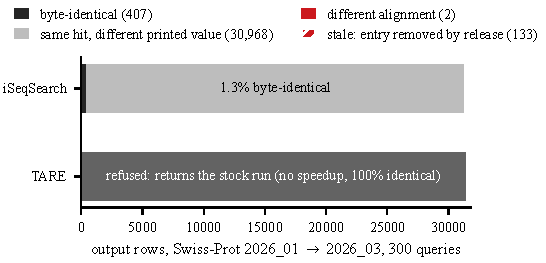
\includegraphics[width=\linewidth]{figures/idiamond.pdf}
\caption{\textbf{Approximate versus exact.} Output of iSeqSearch's incremental DIAMOND after a Swiss-Prot update, compared
line by line with a full run. Its numbers are close, but only 1.3\% of lines match exactly and 133 lines report sequences
the new release deleted. \sys refuses this program and returns the full run.}
% source: MEASURED pipeline/results/reference_diamond/dx.json idiamond.shared_byte_identical=407 idiamond.shared_rows=31377 idiamond.row_extra=133; DERIVED ident_pct=100*shared_byte_identical/shared_rows
\label{fig:idiamond}
\end{figure}

\textbf{Approximate incremental search.} Specialized incremental search does reuse work across a release, but not exactly.
We ran iSeqSearch's incremental DIAMOND~\cite{yoo2025iseqsearch} on the same 300 proteins as our DIAMOND experiment,
updating Swiss-Prot from 2026\_01 to 2026\_03, and compared it with a full run (\cref{fig:idiamond}). Its E-values are close (over 31{,}377 shared lines, Pearson $r = 0.999999$ and Kendall $\tau_b = 0.99999$), but only 407 of those
lines (1.30\%, Wilson 95\% CI 1.18--1.43\%) are byte-identical; 30{,}968 report the same
alignment with different printed numbers, 2 report a different alignment, and 133 lines are hits to sequences the new
release removed. \sys refuses this program and returns the full run; where it replays, every line is identical.
% source: MEASURED pipeline/docs/EXACT_REPLAY_PROTOCOL.md; TEXT q300=300; MEASURED pipeline/results/reference_diamond/dx.json idiamond.shared_rows=31377 idiamond.evalue_pearson=0.9999991687961751 idiamond.evalue_kendall_tau=0.9999939628622326 idiamond.shared_byte_identical=407 idiamond.same_hsp_different_value=30968 idiamond.different_hsp=2 idiamond.row_extra=133; DERIVED ident_pct=100*shared_byte_identical/shared_rows; DERIVED wlo=100*wilson_lo(shared_byte_identical,shared_rows); DERIVED whi=100*wilson_hi(shared_byte_identical,shared_rows); NOMINAL ci=95

\textbf{Record-side reuse.} The same machinery applies when the \textit{proteins}, not the database, are new. On SnpEff
variant annotation~\cite{cingolani2012snpeff}, reusing earlier records gave a speedup of $1.17\times$ on a dedicated node (median of 10 alternating paired ratios; 95\%
percentile bootstrap CI 1.159--1.171 from 10{,}000 resamples, which lies above the stock time), with byte-identical output on 52{,}638 records. A laptop fit of the same startup model gives $1.35\times$; that fit is not the node measurement. On HMMER over
collections of 30 and 40 \textit{E.~coli} genomes, reusing proteins searched earlier gave cumulative speedups (M5, ratio of summed times) of $2.04\times$ and $4.94\times$, or $1.66\times$
and $3.53\times$ including the one-time probe cost $P = 1{,}595$\,s.
% source: MEASURED pipeline/results/snpeff_alternating_carc.json median_r=1.166822900685488 bootstrap.n=10000 bootstrap.ci95_lo=1.1594572565112815 bootstrap.ci95_hi=1.1705137290260232 locked.N=52638; LEN pairs=10; MEASURED pipeline/results/snpeff_timing_fit.json prediction.speedup=1.3485471039049597; MEASURED pipeline/results/savings_measured_hmmsearch.json collections.A.n_genomes=30 collections.B.n_genomes=40 collections.A.cum_speedup_wall=2.036508804084894 collections.B.cum_speedup_wall=4.936408335087653 collections.A.cum_speedup_wall_with_P=1.6596265417942682 collections.B.cum_speedup_wall_with_P=3.5331974513289715 collections.A.probe_wall_s=1595.4474956459528; NOMINAL ci=95

% =====================================================================
\section{Discussion}
\label{sec:discussion}

\textbf{Threats to validity.} \textit{Generality:} the two programs \sys replays exactly, HMMER and Infernal, come from one
research group and share code, so they may share the property that makes replay work; the two refused programs come from
other groups. We therefore claim that the method works for programs whose coupling lies in settings they expose, and that
it detects when coupling lies elsewhere; we do not claim it works for most search programs. \textit{Release choice:} we
measure one release pair per database; smaller releases should be faster, as the model projects, but we have not measured
them. \textit{Timing:} workstation numbers are single runs on a shared machine; the headline is measured on a dedicated
node with alternating runs. \textit{Check strength:} the random pads are weak (\cref{fig:pmiss}).

\textbf{Anticipated objections.} \textit{``Why not just rescale the cached E-values?''} Rescaling reproduces the program's
arithmetic but not its rounding, and it must be written for each program and column; pinning lets the program print its
own numbers. \textit{``InterProScan already reuses precomputed results.''} Its lookup is keyed by the protein sequence for
a fixed database version; it answers ``has this protein been seen?'' rather than ``what changed in the database?''
\textit{``Use a faster or GPU search program.''} That is complementary: it shrinks $T_{\text{stock}}$, and \sys's savings
apply on top whenever the program's coupling can be pinned.

\textbf{Deployment.} The natural deployment is InterProScan~\cite{jones2014interproscan} after a member-database update.
Member databases that score each model against its own threshold, as Pfam does, should behave like our HMMER results;
those that compare hits across models would need declared groups or would be refused.

% =====================================================================
\section{Related Work}
\label{sec:related}

\begin{table*}[t]
\caption{Prior work on the problem of updating annotations after a database release. ``Unmodified'': runs the program as
is. ``Release-aware'': reuses work when the database changes. ``Identical'': output equals a full run byte for byte.
``Per-tool code'': requires code or formulas written for each program.}
\label{tab:prior}
\centering\footnotesize
\setlength{\tabcolsep}{3.5pt}
\begin{tabular}{@{}llcccc>{\raggedright\arraybackslash}p{3.6cm}@{}}
\toprule
System & Grain & Unmodified & Release-aware & Identical & Per-tool code & Limitation for this problem \\
\midrule
Riker, ProcessCache, INCR~\cite{curtsinger2022riker,shiptoski2023processcache,xie2026incr} & command / chunk & yes & no & yes & no & a release reruns everything \\
Nextflow, Snakemake~\cite{ditommaso2017nextflow,molder2021snakemake} & task & yes & no & yes & no & task inputs change \\
iBLAST~\cite{dash2021iblast} & appended sequences & yes & growth only & rescaled & yes & BLAST-specific E-value formula \\
iSeqSearch~\cite{yoo2025iseqsearch} & appended sequences & yes & growth only & rescaled & yes & 1.3\% of lines identical; stale hits \\
% source: MEASURED pipeline/results/reference_diamond/dx.json idiamond.shared_byte_identical=407 idiamond.shared_rows=31377; DERIVED ident_pct=100*shared_byte_identical/shared_rows
GeStore~\cite{pedersen2014gestore} & plugin & yes & yes & rescaled & yes & administrator-written plugins \\
Precomputed lookups~\cite{jones2014interproscan,cantalapiedra2021eggnog} & query sequence & yes & no & yes & no & keyed by query, fixed release \\
KumQuat~\cite{shen2022kumquat} & input stream & yes & no & yes & no & no database argument \\
IVM, self-adjusting~\cite{blakeley1986views,acar2003selective} & operator & no & yes & yes & n/a & computation must be rewritten \\
\sys & record $\times$ entry & yes & yes & yes & no & refuses programs with hidden coupling \\
\bottomrule
\end{tabular}
\end{table*}

\textbf{General-purpose incremental execution.} Build systems and workflow managers avoid repeated work by keying a command
on the bytes it reads (\cref{tab:prior}). Riker traces system calls to rerun only commands whose inputs
changed~\cite{curtsinger2022riker}; ProcessCache caches process executions~\cite{shiptoski2023processcache}; INCR memoizes
shell command effects and can split inputs into annotated chunks~\cite{xie2026incr}; Nextflow, Snakemake, and Cromwell hash
task inputs~\cite{ditommaso2017nextflow,molder2021snakemake,cromwell-call-cache}; and Mokhov et al.\ model the design
space~\cite{mokhov2018buildsystems}. Their unit of reuse is the command, so they cannot reuse part of an output whose
numbers depend on the whole database. \sys is complementary: it decides what to rerun inside one command.

\textbf{Incremental sequence search.} iBLAST searches only appended sequences and corrects BLAST's E-values with a formula
derived for BLAST~\cite{dash2021iblast}. iSeqSearch applies that correction to other programs with BLAST-style output,
including DIAMOND~\cite{yoo2025iseqsearch}. GeStore runs unmodified BLAST and HMMER through administrator-written plugins
that rewrite inputs and merge outputs~\cite{pedersen2014gestore}. MMseqs2 supports incremental
clustering~\cite{steinegger2017mmseqs2}, and InterProScan and eggNOG-mapper reuse precomputed matches keyed by protein
sequence~\cite{jones2014interproscan,cantalapiedra2021eggnog}. These approaches are hand-built for one program, approximate
when the database changes, or keyed by query rather than database. Our DIAMOND result applies directly to them: no
correction of DIAMOND's printed numbers can recover hits its filter dropped because a neighboring entry was absent.

\textbf{Black-box decomposition and incremental computation.} KumQuat synthesizes combiners that let an unmodified command
run on pieces of its input stream~\cite{shen2022kumquat}, and Caruca classifies opaque commands by whether they keep
state~\cite{lamprou2025caruca}. Incremental view maintenance and self-adjusting computation keep results current under
input changes but require the computation to be written in their framework~\cite{blakeley1986views,acar2003selective}.
These methods split an input stream or a known program; \sys splits a database argument whose size enters every printed
number, for a binary it cannot inspect. Its partition probes borrow the spirit of metamorphic
testing~\cite{chen1998metamorphic,segura2016survey} rather than claiming a new testing method.

% =====================================================================
\section{Conclusion}
\label{sec:conclusion}

Reference databases change every few weeks to months, and the programs that search them start from scratch every time. We
showed that for an important class of programs this is unnecessary: the coupling between database entries lies in a few
numbers the program already lets users set, and pinning those numbers lets an unmodified program reprint, byte for byte, the
output of a full run while searching only what changed. \sys discovers that coupling, replays exactly where it can, and
refuses where it cannot, as it did for DIAMOND, whose filter reads neighboring entries. Every output \sys produced across
HMMER and Infernal was identical to a full rerun, and a Pfam update ran \pending{X$\times$} faster than a full rerun on a
dedicated server. Extending \sys to InterProScan's member databases, and sizing its check by sequence length rather than
record count, are the next steps.

\section*{Availability}
An anonymized artifact accompanies this submission. It contains \sys, every pre-registration and addendum, the result files
from which each number in this paper is taken, and the scripts that regenerate every figure from those files. The repository
URL is omitted for double-blind review.

\bibliographystyle{plain}
\bibliography{refs}

\end{document}
